\documentclass[12pt]{article}

\usepackage{polski}			% Polish characters
\usepackage[utf8]{inputenc}	% Polish characters
\usepackage{indentfirst}	% Indentation in first paragraph
\usepackage{graphicx}
\usepackage{geometry}
\usepackage{hyperref}

	
\graphicspath{{images}} %Setting the graphicspath

\hypersetup{
	linkcolor=black,
	colorlinks=true,
	urlcolor=blue,
	}
\urlstyle{same}

\begin{document}


\begin{titlepage} % Titlepage don't count to page numbering
	
	\center % Centre everything on the page
	
	%----------------------------------------------------------------------------------------
	%	Title
	
	\rule[1.0cm]{\textwidth}{1.0mm}
	
	{\huge\bfseries Olympus Movie}\\[0.5cm]
	
	\rule[1.5cm]{\textwidth}{1.0mm}
	%----------------------------------------------------------------------------------------	
	
	%----------------------------------------------------------------------------------------
	%	Logo
	
	
\includegraphics[scale=0.5]{logo.png}\\[1cm]
	
	%----------------------------------------------------------------------------------------
	
	%----------------------------------------------------------------------------------------
	%	Author(s)
	
	\begin{minipage}{0.4\textwidth}
		\begin{flushright}
			\large
			\textit{Autorzy}\\
			Jakub Nowak
			
			Marcelina Ziętal
			
			Dawid Polaczek
		\end{flushright}
	\end{minipage}
	%----------------------------------------------------------------------------------------
	
	%----------------------------------------------------------------------------------------
	%	Date
	
	\vspace{\fill}
	2022
	
	%----------------------------------------------------------------------------------------
	
	
\end{titlepage}
\newgeometry{tmargin=2.5cm, bmargin=2.5cm, lmargin=3cm, rmargin=1.5cm}
	%----------------------------------------------------------------------------------------
	%	Table of contents
	
	\tableofcontents
	\pagebreak
	%----------------------------------------------------------------------------------------
	
	%----------------------------------------------------------------------------------------
	%	Chapters

	\section{Słownik}	%rozpisać skróty i ujednolicić dokumentację
		
	\section{Specyfikacja wymagań biznesowych}
	
		\subsection{Cel systemu}	%opis dlaczego taki system i jakie problemy rozwiazuje jego zbudowanie 
		Celem projektu "Olympus Movie" jest stworzenie strony internetowej poświęconej filmom, serialom oraz osobom uczestniczącym w ich tworzeniu. Użytkownik po zarejestrowaniu i zalogowaniu jest w stanie komentować, oceniać i recenzować pozycje.
	
	Każda osoba odwiedzająca stronę ma możliwość wyszukania pozycji na podstawie licznych filtrów. Podstawowe wyszukiwanie przeszukuje jedynie tytuły. Istniej możliwość wyszukiwania zaawansowanego w którym wyszukiwanie następuje po tagach lub gatunkach.
	
	Baza danych zawiera również informacje o aktorach, reżyserach i scenarzystach. Pozwala to na wyświetlenie filmów w których grał konkretny aktor lub konkretna osoba brała udział w jego tworzeniu.
		
		\subsection{Wymagania funkcjonalne}
			\begin{itemize}
				\item Wyszukiwanie filmów/seriali
				\item Możliwość utworzenia konta
				\item Dodawanie recenzji lub oceny danego filmu lub serialu
				\item Tworzenie listy obejrzanych filmów oraz seriali
				\item Filtrowanie i sortowanie filmów lub seriali według wybranych kryteriów
			\end{itemize}
		
		\subsection{Wymagania niefunkcjonalne}
			\begin{itemize}
				\item Korzystanie z serwisu za pośrednictwem przeglądarki internetowej
				\item Kompatybilność z przeglądarkami obsługującymi HTML 5
				\item Przejrzysty interfejs użytkownika
				\item Szybka reakcja na działania użytkownika
				\item Zapewnienie ciągłości dostępu do serwisu użytkownikom
			\end{itemize}
		
		\subsection{Opis ograniczeń systemu}
			\subsubsection{Odtwarzanie trailerów}
				\begin{enumerate}
					\item Trailery oraz plakaty wyświetlane na stronie nie znajdują się w bazach danych. Przechowywane są jedynie linki do nich ze stron zewnętrznych.
					\item Brak listy znajomych lub obserwowanych użytkowników \
					\item Brak powiadomień.
					\item Brak ustawień. W tym zmiany języka
					%\item Brak zmiany motywu na stronie
					\item Mocno ograniczony zakres bazy danych. Serwis nie posiada możliwości importowania pozycji z zewnętrznej strony. Wszystkie dane muszą zostać wprowadzone bezpośrednio w serwisie.
				\end{enumerate}
						
			
				
				
				
				
				 
%			\begin{itemize}
%				\item Trailery 
%			\end{itemize}

%Trailer i plakat ma link. Nie am tego w bazie danych
%brak listy znajomych/obserwowanych
%brak powiadomień
%Brak ustawień - zmiany języka itp.
%Brak zmianu motywu na stronie
%Niepełna baza danych
		
	\section{Dokumentacja techniczna}
	
		\subsection{Architektura systemu}
%mikroserwisy
		
		\subsection{Diagramy przypadków użycia}
			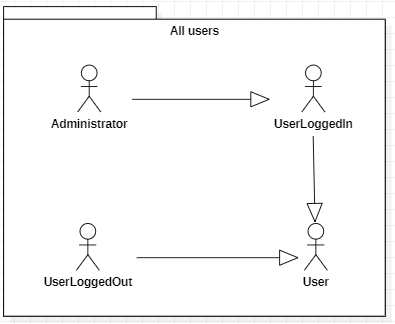
\includegraphics[scale=0.9]{UseCase_AllUsers.png} \linebreak
			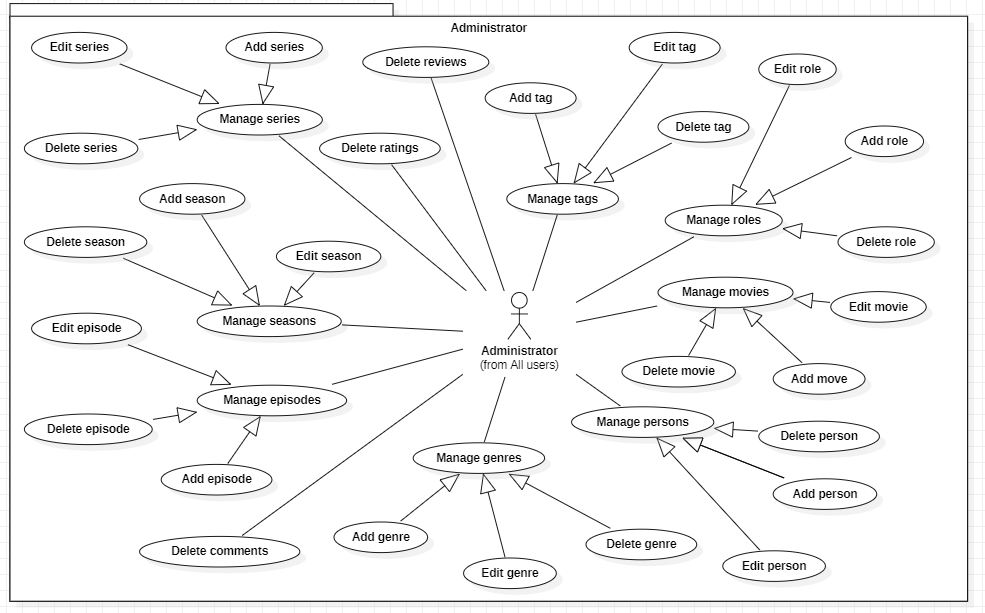
\includegraphics[scale=0.7]{UseCase_Administrator.png} \linebreak
			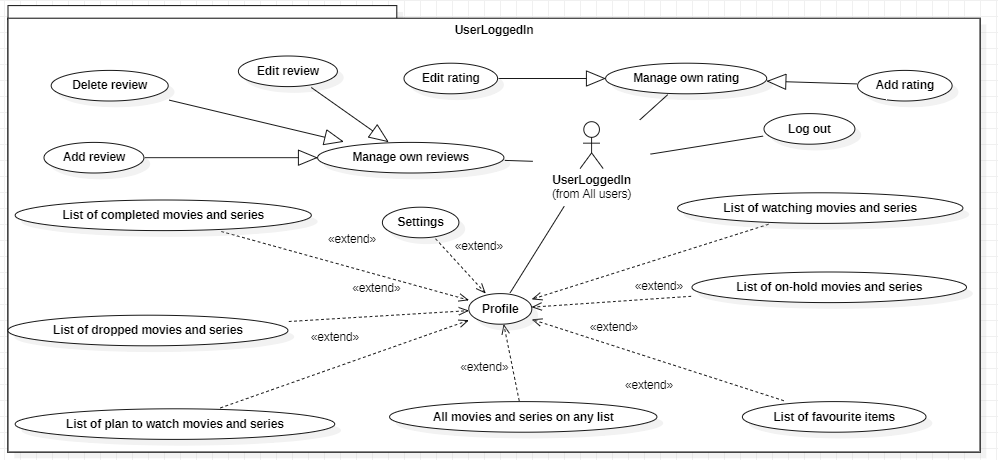
\includegraphics[scale=0.7]{UseCase_UserLoggedIn.png} \linebreak
			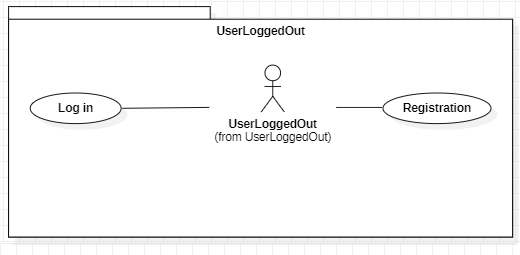
\includegraphics[scale=0.9]{UseCase_UserNotLoggedIn.png} \linebreak
			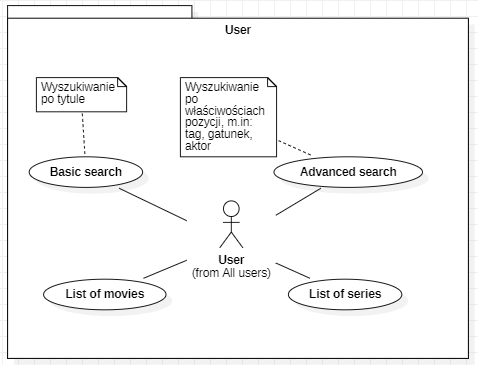
\includegraphics[scale=0.9]{UseCase_User.png} \linebreak
		
		\subsection{Diagram klas}
			\begin{center}
				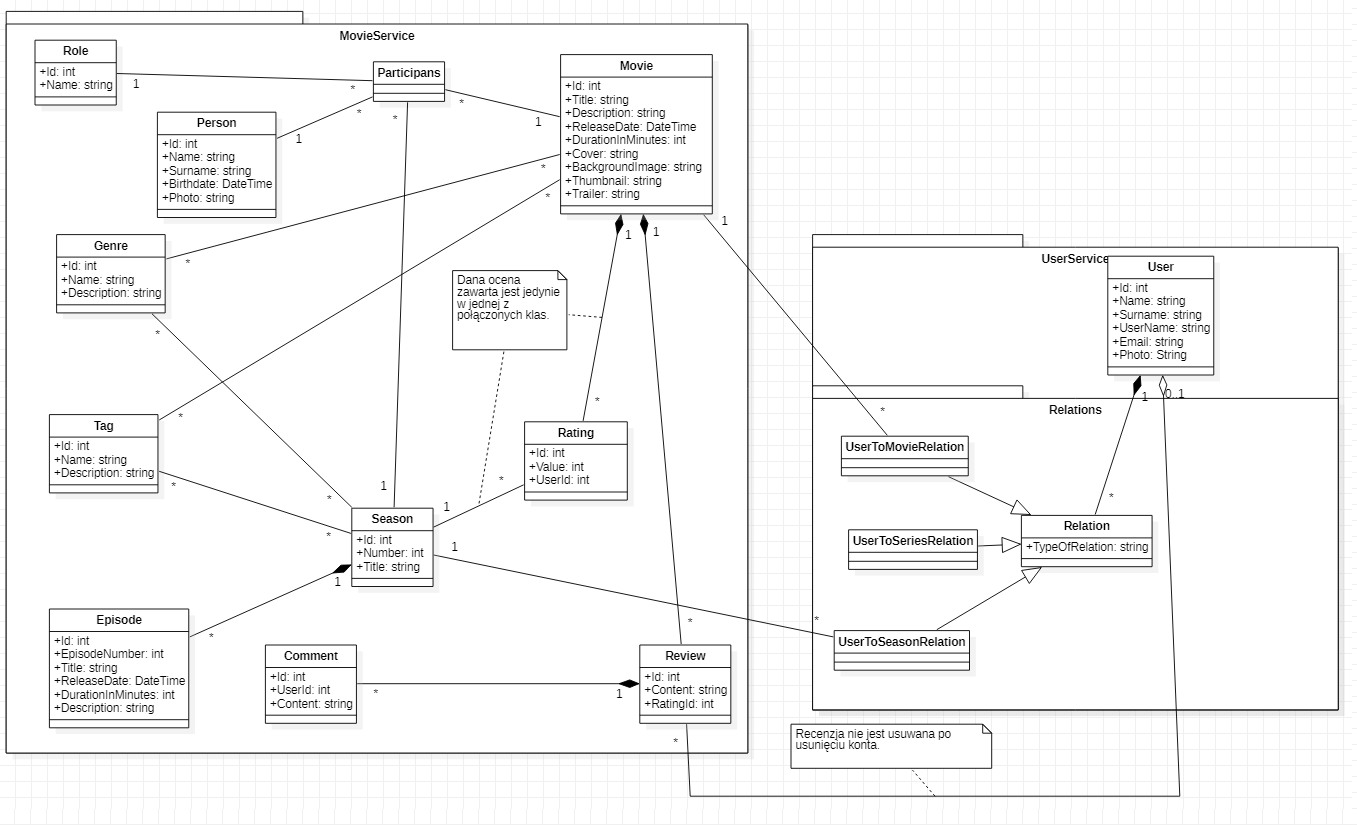
\includegraphics[scale=0.5]{Class_FilmsDataBase.png}
			\end{center}
		
		\subsection{Dokumentacja API}	%swaggers
			
	\section{Dokumentacja użytkownika}
		\subsection{Funkcjonalność użytkownika anonimowego}
%		
		\subsection{Funkcjonalność użytkownika zalogowanego}
%		
%		\subsection{Funkcjonalność użytkownika administratora}	
%	
	\section{Informacje o wersji}
	
	


	
	
			
		%\subsection{Mapa strony}
		%\subsection{Lista funkcjonalności}
		%\subsection{Wersje językowe}
	%\section{Wymagania techniczne}
		%\subsection{Wsparcie przeglądarek}
	\pagebreak
	\section{Licencje}
		\begin{enumerate}
			\item	Pixabay
			\url{https://pixabay.com/service/terms/#license}, 
			data ostatniej aktualizacji: 13.12.2021
			
			
			\item	Boxicons
			\url{https://boxicons.com/usage#license}, 
			data wejścia na stronę: 18.10.2022
		\end{enumerate}
	
	
	%----------------------------------------------------------------------------------------
	
	%----------------------------------------------------------------------------------------
	%		Bibliography
%	\bibliographystyle{plain}
%	\bibliography{mybib}
	
	%----------------------------------------------------------------------------------------
\end{document}
